\documentclass[leqno]{article}
\usepackage[utf8]{inputenc}
\usepackage[T1]{fontenc}
\usepackage{amsfonts}
%\usepackage{fourier}
%\usepackage{heuristica}
\usepackage{enumerate}
\author{Colin Roberts}
\title{MATH 570, Homework 11}
\usepackage[left=3cm,right=3cm,top=3cm,bottom=3cm]{geometry}
\usepackage{amsmath}
\usepackage[thmmarks, amsmath, thref]{ntheorem}
%\usepackage{kbordermatrix}
\usepackage{mathtools}
\usepackage{tikz-cd}
\usepackage{ragged2e}

\theoremstyle{nonumberplain}
\theoremheaderfont{\itshape}
\theorembodyfont{\upshape:}
\theoremseparator{.}
\theoremsymbol{\ensuremath{\square}}
\newtheorem{proof}{Proof}
\theoremsymbol{\ensuremath{\square}}
\newtheorem{lemma}{Lemma}
\theoremsymbol{\ensuremath{\blacksquare}}
\newtheorem{solution}{Solution}
\theoremseparator{. ---}
\theoremsymbol{\mbox{\texttt{;o)}}}
\newtheorem{varsol}{Solution (variant)}

\newcommand{\tr}{\mathrm{tr}}
\newcommand{\Int}{\ensuremath{\mathrm{Int}}}
\newcommand{\N}{\ensuremath{\mathbb{N}}}
\newcommand{\Q}{\ensuremath{\mathbb{Q}}}
\newcommand{\R}{\ensuremath{\mathbb{R}}}
\newcommand{\Z}{\ensuremath{\mathbb{Z}}}
\newcommand{\cB}{\ensuremath{\mathcal{B}}}
\newcommand{\cF}{\ensuremath{\mathcal{F}}}
\newcommand{\obj}{\ensuremath{\mathrm{Obj}}}
\newcommand{\im}{\ensuremath{\mathrm{im}}}
\newcommand{\Id}{\ensuremath{\mathrm{Id}}}
\newcommand{\RP}{\ensuremath{\mathbb{RP}}}



\begin{document}
\maketitle
\begin{large}
\begin{center}
Solutions
\end{center}
\end{large}
\pagebreak

%%%%%%%%%%%%%%%%%%%%%%%%%%%%%%%%%%%%%%%%%%%%%%%%%%%%%%%%%%%%%%%%%%%%%%%%%%%%%%%%%%%%%%%%%%%%%%%%%%%%%%%%%%%%%%%%%%%%%
%%%%%%%%%%%%%%%%%%%%%%%%%PROBLEM 1%%%%%%%%%%%%%%%%%%%%%%%%%%%%%%%%%%%%%%%%%%%%%%%%%%%%%%%%%%%%%%%%%%%%%%%%%%%%%%%%%%%%%%%%%%%%%%%%%%%%%%%%%%%%%%%%%%%%%%%%%%%%%%%%%%%%%%%%%%%%%%%%%%%%%%%%%%%%%%%%%%%%%%%%%%%%%%%%%%%%%%%%%%%%%%%%%%%%%%%%

\noindent\textbf{Problem 1.} Let $X$ be the 2-dimensional simplicial complex with ten 2-simplices drawn below; recall that $X$ is homeomorphic to the projective plane $\RP^2$.
\begin{center} 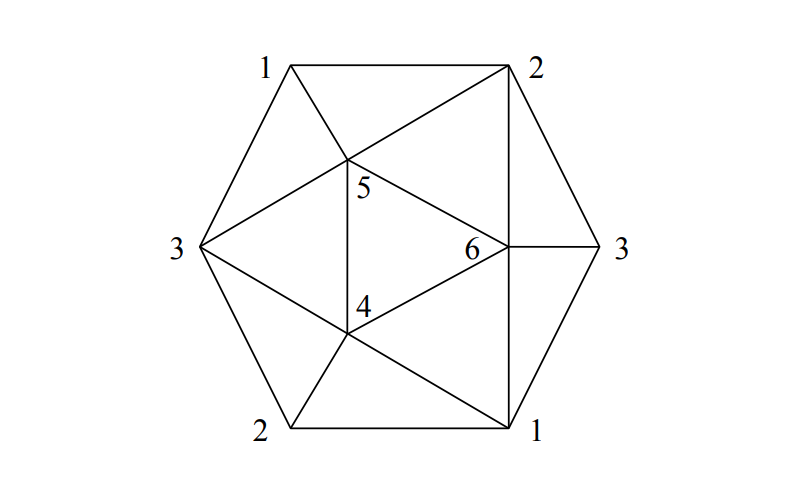
\includegraphics[width=2in]{projective_plane.png} \end{center}
Show that the 2-dimensional simplicial homology group of $X$ is $H_2(X)\cong0$.

\noindent\rule[0.5ex]{\linewidth}{1pt}

\begin{proof}
Henry has a hint online.
\end{proof}

\pagebreak

%%%%%%%%%%%%%%%%%%%%%%%%%%%%%%%%%%%%%%%%%%%%%%%%%%%%%%%%%%%%%%%%%%%%%%%%%%%%%%%%%%%%%%%%%%%%%%%%%%%%%%%%%%%%%%%%%%%%%
%%%%%%%%%%%%%%%%%%%%%%%%%PROBLEM 2%%%%%%%%%%%%%%%%%%%%%%%%%%%%%%%%%%%%%%%%%%%%%%%%%%%%%%%%%%%%%%%%%%%%%%%%%%%%%%%%%%%%%%%%%%%%%%%%%%%%%%%%%%%%%%%%%%%%%%%%%%%%%%%%%%%%%%%%%%%%%%%%%%%%%%%%%%%%%%%%%%%%%%%%%%%%%%%%%%%%%%%%%%%%%%%%%%%%%%%%


\noindent\textbf{Problem 2.} Prove Proposition~13.5 in our book: If $X$ is a space, $\{X_\alpha\}_{\alpha \in X}$ is the set of path components of $X$, and $\iota_\alpha\colon X_\alpha\hookrightarrow X$ is the corresponding inclusion, then for each $p\ge0$ the map $\oplus_{\alpha\in A}H_p(X_\alpha)\to H_p(X)$ whose restriction to singular homology group $H_p(X_\alpha)$ is $(\iota_\alpha)_*\colon H_p(X_\alpha)\to H_p(X)$ is an isomorphism. Proceed by the following steps.
\begin{enumerate}[(a)]
\item Show the maps $(\iota_\alpha)_\#\colon C_p(X_\alpha)\to C_p(X)$ give an isomorphism $g_C\colon\oplus_{\alpha\in A}C_p(X_\alpha)\to C_p(X)$, defined by $g_C((c_\alpha)_{\alpha\in A})=\sum_\alpha(\iota_\alpha)_\#(c_\alpha)$, where $c_\alpha\in C_p(X_\alpha)$. Injectivity is clear, and the first sentence of the proof in our book implies surjectivity.
\item Show that restricting $g_C$ gives an isomorphism $g_Z\colon\oplus_{\alpha\in A}Z_p(X_\alpha)\to Z_p(X)$. The injectivity of $g_Z$ follows from that of $g_C$; you need to show that $g_Z$ is well-defined and surjective.
\item Show that restricting $g_C$ gives an isomorphism $g_B\colon\oplus_{\alpha\in A}B_p(X_\alpha)\to B_p(X)$. The injectivity of $g_B$ follows from that of $g_C$; you need to show that $g_B$ is well-defined and surjective.
\item Deduce that $g_C$ induces an isomorphism $\oplus_{\alpha\in A}H_p(X_\alpha)\to H_p(X)$.
\end{enumerate}


\noindent\rule[0.5ex]{\linewidth}{1pt}

\begin{proof}
\begin{enumerate}[(a)]
\item 

\end{enumerate}
\end{proof}


\pagebreak


%%%%%%%%%%%%%%%%%%%%%%%%%%%%%%%%%%%%%%%%%%%%%%%%%%%%%%%%%%%%%%%%%%%%%%%%%%%%%%%%%%%%%%%%%%%%%%%%%%%%%%%%%%%%%%%%%%%%%
%%%%%%%%%%%%%%%%%%%%%%%%%PROBLEM 3%%%%%%%%%%%%%%%%%%%%%%%%%%%%%%%%%%%%%%%%%%%%%%%%%%%%%%%%%%%%%%%%%%%%%%%%%%%%%%%%%%%%%%%%%%%%%%%%%%%%%%%%%%%%%%%%%%%%%%%%%%%%%%%%%%%%%%%%%%%%%%%%%%%%%%%%%%%%%%%%%%%%%%%%%%%%%%%%%%%%%%%%%%%%%%%%%%%%%%%%


\noindent\textbf{Problem 3.}  Prove Proposition~13.6: For any topological space $X$, the singular homology group $H_0(X)$ is a free abelian group with basis consisting of an arbitrary point in each path component.

\emph{Remark: Our book contains a detailed proof; you can learn and use this proof!}

\noindent\rule[0.5ex]{\linewidth}{1pt}

\begin{proof}
First, assume $X$ is path-connected.  Let an element in $C_0$ be given by $c=\sum_{i=1}^m$ and define the map $\epsilon \colon C_0(X)\to \Z$ by
\[
\epsilon \left( \sum_{i=1}^m n_i x_i \right) = \sum_{i=1}^m n_i.
\]
Clearly, $\epsilon$ is a surjective group homomorphism.  

Now choose a point $x_0\in X$ and for every $x\in X$ let $\alpha(x)$ be a path from $x_0$ to $x$.  This path $\alpha$ is a singular $1$-simplex whose boundary is the $0$-chain $x-x_0$.  So for an arbitrary $0$-chain $c$, we have
\[
\partial \left( \sum_{i=1}^m \alpha(x_i) \right) = \sum_{i=1}^m - \sum_{i=1}^m n_i x_0=c-\epsilon(c)x_0.
\]
If we then let $c\in \ker\epsilon$ so that $\epsilon(c)=0$ we find that $c\in B_0(X)$. This means that $\ker\epsilon \subseteq B_0(X)$.

Next, note that $B_0(X)\in \ker \epsilon$ since for any singular $1$-simplex $\sigma$ we have $\partial \sigma = \sigma(1)-\sigma(0)$ and in particular, $\epsilon(\partial\sigma)=1-1=0$.  This means $B_0(X)\subseteq \ker \epsilon$.  

Then we have that $\ker\epsilon = B_0(X)$, and by the first isomorphism theorem, that $\epsilon$ induces and isormorphism $H_0\to \Z$.  Finally, by Proposition 13.5, we have that $H_0(X)$ is a direct sum of infinite cyclic groups, one for each path component.  Hence, we have $H_0(X)$ is a free abelian group with basis consisting of an arbitrary point in each path component. 
\end{proof}

\pagebreak



%%%%%%%%%%%%%%%%%%%%%%%%%%%%%%%%%%%%%%%%%%%%%%%%%%%%%%%%%%%%%%%%%%%%%%%%%%%%%%%%%%%%%%%%%%%%%%%%%%%%%%%%%%%%%%%%%%%%%
%%%%%%%%%%%%%%%%%%%%%%%%%PROBLEM 3%%%%%%%%%%%%%%%%%%%%%%%%%%%%%%%%%%%%%%%%%%%%%%%%%%%%%%%%%%%%%%%%%%%%%%%%%%%%%%%%%%%%%%%%%%%%%%%%%%%%%%%%%%%%%%%%%%%%%%%%%%%%%%%%%%%%%%%%%%%%%%%%%%%%%%%%%%%%%%%%%%%%%%%%%%%%%%%%%%%%%%%%%%%%%%%%%%%%%%%%


\noindent\textbf{Problem 4.}  Use the Mayer-Vietoris Theorem to prove Theorem~13.23: For $n\ge 1$, the singular homology groups of the sphere $S^n$ are
\[ H_p(S^n)\cong\begin{cases}
\Z &\mbox{if }p=0\mbox{ or }n\\
0 &\mbox{if }0<p<n\mbox{ or }p>n.
\end{cases} \]

\emph{Remark: Our book contains a detailed proof; you can learn and use this proof!}

\noindent\rule[0.5ex]{\linewidth}{1pt}

\begin{proof}
We let $N$ and $S$ represent the north and south poles of $S^n$.  Now $U=S^n\setminus \{N\}$ and $V=S^n\setminus \{S\}$.  Since $U$ and $V$ are contractible, the Mayer Vietoris sequence is
\[
0 \to H_p(S^n)\xrightarrow{\partial_*} H_{p-1}(U\cap V) \to 0,
\]
which gives us that $\partial_*$ is an isomorphism.  Since $U\cap V$ is homotopy equivalent to $S^{n-1}$,
\[
H_p(S^n)\cong H_{p-1}(U\cap V) \cong H_{p-1}(S^{n-1}) ~~ \textrm{for} ~p>1, n\geq 1.
\]
Now we finish by induction.  For the case $n=1$, $H_0(S^1)\cong H_1(S^1)\cong \Z$ by Proposition 13.6 and Corollary 13.15. For $p>1$, The Mayer Vietoris theorem tells us that $H_p(S^1)\cong H_{p-1}(S^0)$. Since $S^0$ is the disjoint union of two points, $H_{p-1}(S^0)$ is the trivial group by Propositions 13.7 and 13.5.

Next, suppose the result is true for $S^{n-1}$ for $n>1$, then for $p=0$ and $p=1$ we have the result by Proposition 13.6 and Corollary 13.15. For $p>1$, the Mayer Vietoris theorem and the inductive hypothesis imply that
\[
H_p(S^n)\cong H_{p-1}(S^{n-1})\cong 
\begin{cases}
0 & \textrm{if}~ p<n, \textrm{or} p>n,\\
\Z & \textrm{if}~ p=n.
\end{cases}
\]
Hence, we are finished.
\end{proof}

\end{document}

